\section{Implementation on SonarJava}
\label{sec:implementation_java}

We are first going to implements this check on the SonarJava ecosystem that already provide us all the tools that we need, specifically symbols resolutions, and a control flow graph.
The implementation is a classical forward data-flow analysis: the first step is to generate for each basic block the gen and kill set as described before. 
We are going to store the symbols of the variable in the two set. 
We fill the set going top-down in the elements of the basic block, when a pointer is killed, we also remove it if it is present in the gen set. 
With this, a pointer that is used and assigned in the same basic block will be in gen set only if the use of the pointer follow the assignment, as expected.

\lstinputlisting[label={lst:native-block-creation},
caption=Problematic situation with naive basic block creation]{code/native-block-creation.scala} 

Listing \ref{lst:native-block-creation} shows a potential problem of this method, all the different parts of the code will be added to the same basic block, we will therefore have a situation that we would want to report, but is not detected since the pointer is not in the gen set of this block. 
One naive solution would be to not aggregate statements in basic block, but we will have to compute the input and output set for every statements! [TODO: ev explain performance diff]
The alternative that we use in this work is done during the control flow graph creation: we break the basic block when we have a binary expression with an equals (or not equals). 
In order to support the backward and forward analysis, we should break before and after the check for null. 
We can now safely consider that a pointer that is checked will never be in the same basic block as where it is used or killed.
\begin{figure}[h]
\caption{Example of the new way to split basic block}
\label{figure:new-way-to-split}
\setlength{\tabcolsep}{24pt}
	\begin{tabular}{cc}
		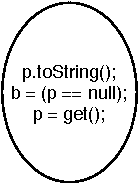
\includegraphics[]{figure/original-block-cfg.pdf}  &
		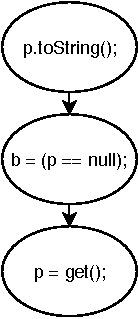
\includegraphics[]{figure/splitted-block-cfg.pdf}   \\ 
		Original block & Splitted block
	\end{tabular}
\end{figure}

Figure \ref{figure:new-way-to-split} shows the old and new control flow graph for the code of listing \ref{lst:native-block-creation}. 
By doing this, we will be able to support the examples shown in listing \ref{lst:native-block-creation}, the check for null break the block in three, the use and check will therefore not be in the same basic block.

Once the \emph{gen} \ref{eqn:dataflow3} and \emph{kill} \ref{eqn:dataflow4} set has been generated for every basic block, we can start to run the analysis with a work list approach.
The idea is to add all basic block in a queue, compute the new out set of the current head. 
Since we are performing a forward analysis, if the new out set have changed, this means that all the successor might potentially change as well. 
We therefore add the current basic block and all of it successor at the end of the work list. 
We continue this process until the list is empty.

Finally, after having reached a fixed point, we have a set of pointer that are believed to not be null in each basic block.
We can therefore do a second pass through the elements of the basics block, if we see a check for \emph{null} (implies that this pointer could be \emph{null}) in a block where the pointer is in the set of believed to not be \emph{null}, we have a contradiction and report an issue.

\subsection{Other way to add belief}
\label{subsec:other_way_to_add_belief}

Null pointer exception does not occurs only when a null pointer is dereferenced, but can also appear in the following cases for java, as defined in the Java documentation \cite{OracleDoc:2019:Online}:

\begin{enumerate}
	\item Calling the instance method of a null object. \newline 
	\item Accessing or modifying the field of a null object. \newline 
	\item Taking the length of null as if it were an array. \newline 
	\item Accessing or modifying the slots of null as if it were an array. \newline 
	\item Throwing null as if it were a throwable value. \newline 
\end{enumerate}

Currently, our checker is only using the first case, but we can use this information to improve our implementation: when we see one of these construct, we will add the pointer to the set of believed to be non-null (\emph{gen} set) the same way as we would for a pointer that is used.


